%! Author = Len Washington III
%! Date = 09/29/2023

% Preamble
\documentclass[12pt]{report}

% Packages
\usepackage[title={Sep 29, 2023 Notes}]{math252notes}
\usepackage{amssymb}
% Document
\begin{document}

\setcounter{chapter}{4}
\chapter[Modeling with Higher-Order DEs]{Modeling with Higher-Order Differential Equations}\label{ch:modeling-with-higher-order-differential-equations}
\setcounter{section}{0}
%<*Section-5.1>
\section{Spring-Mass Problems}\label{sec:spring-mass-problems}
Suppose that there are no forces affecting the motion other than the gravitational force and the spring force.\\

\begin{figure}[H]
	\centering
	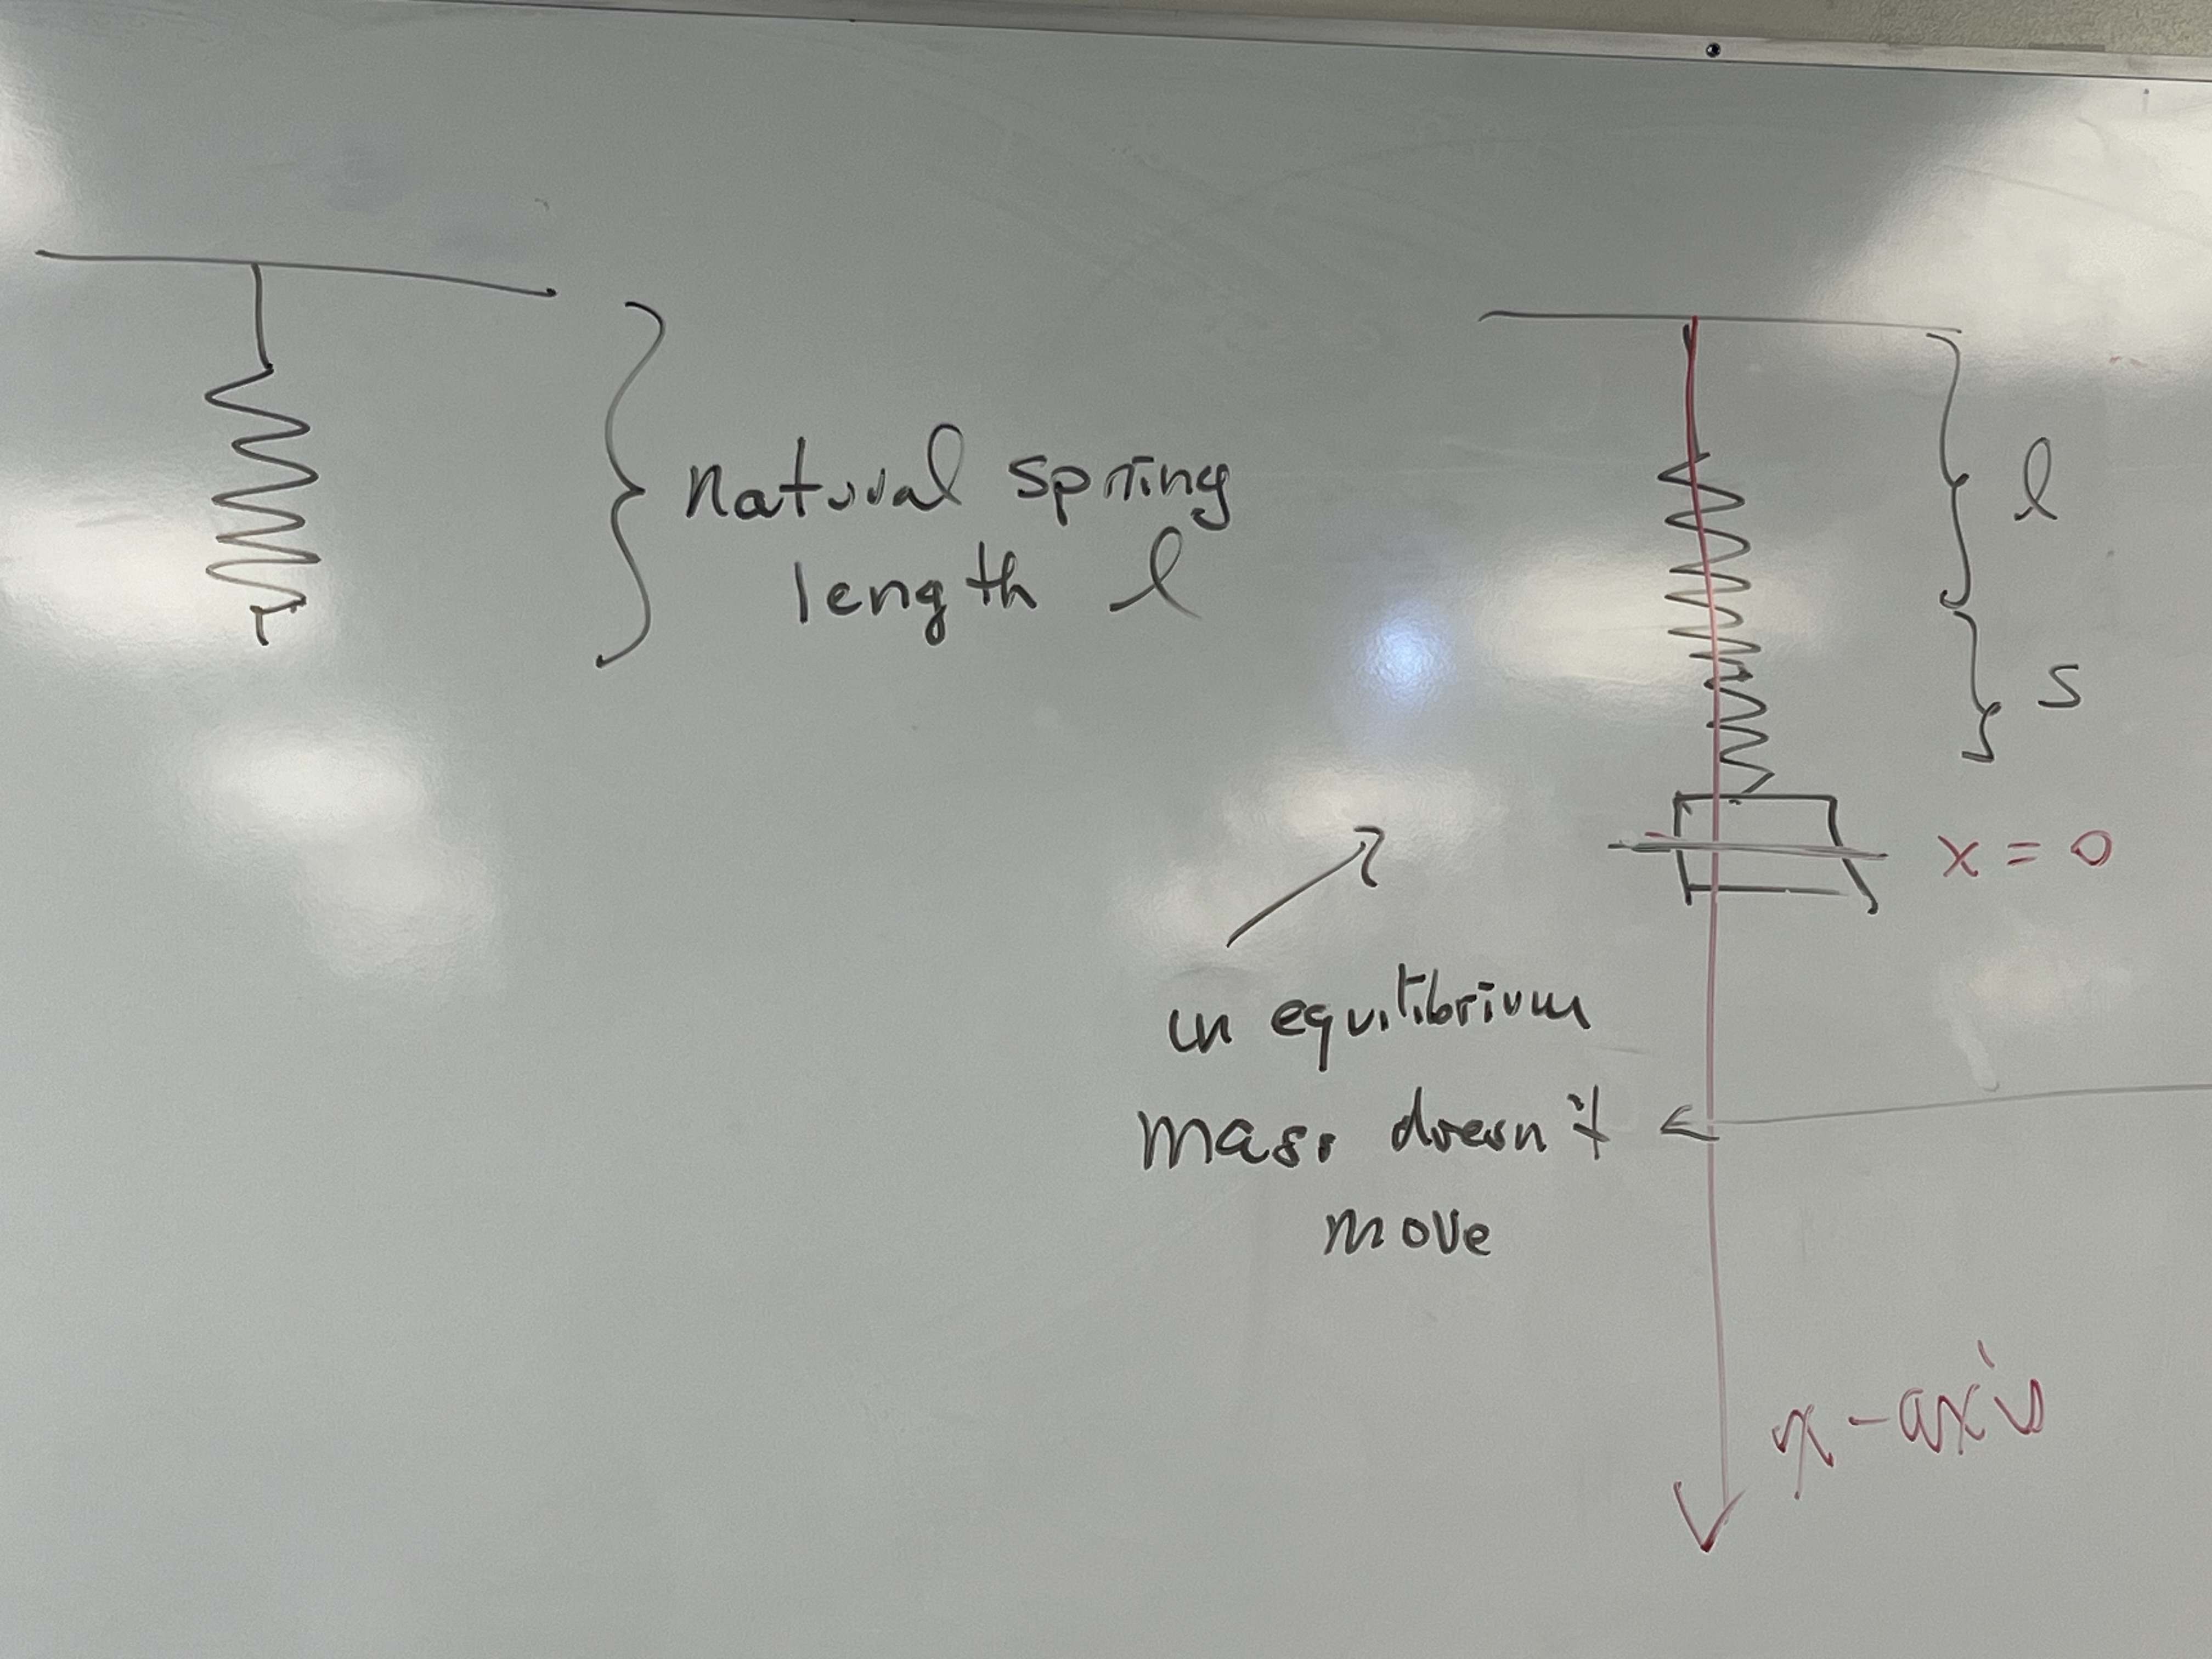
\includegraphics[width=\textwidth]{5.1.spring}
	\caption{Diagram of a spring in equilibrium.}
	\label{fig:5.1.spring}
\end{figure}


In Equilibrium, mass doesn't move.
\[ F_{g} = -F_{spring} \rightarrow mg = -F_{spring} \rightarrow -mg = -kx (\mbox{Hooke's Law})\]
where $g\approx 9.8 m/s^{2}$ if m is in kg, else $g\approx 32.1 ft/sec^{2}$.\\

In equilibrium: \[ F_{net} = mg - ks = 0 \], so \[ k = \frac{mg}{s} \]

In general: \[ F_{net} = m\times acceleration \rightarrow m\frac{d^{2}x}{dt^{2}} \]
\begin{equation*}
\begin{aligned}
	mg + (-k)(x+s) &= m\frac{d^{2}x}{dt^{2}}\\
	mg -kx - ks &= m\frac{d^{2}x}{dt^{2}}\\
	(mg - ks) - kx &= m\frac{d^{2}x}{dt^{2}}\\
	0 - kx &= m\frac{d^{2}x}{dt^{2}}\\
\end{aligned}
\end{equation*}

So the differential equation is: \begin{equation}\label{eq:spring-de} m\frac{d^{2}x}{dt^{2}} + kx = 0 \end{equation}, a 2nd order, homogeneous DE with a constant coefficient.

\example
\begin{equation*}
\begin{aligned}
	m\frac{d^{2}x}{dt^{2}} + kx &= 0\\
	\frac{d^{2}x}{dt^{2}} + \frac{k}{m}x &= 0\\
\end{aligned}
\end{equation*}

Guess: \[ x = e^{lt} \]

\begin{equation*}
\begin{aligned}
	m\frac{d^{2}x}{dt^{2}} + kx &= 0\\
	l^{2}e^{lt} + \frac{k}{m}e^{lt} &= 0\\
	l^{2} + \frac{k}{m} &= 0\\
	l^{2} &= -\frac{k}{m}\\
	l &= \pm\sqrt{-\frac{k}{m}}\\
	l &= 0\pm\sqrt{\frac{k}{m}}i
\end{aligned}
\end{equation*}\begin{equation*}
\begin{aligned}
	x_{1} &= e^{0t}\cos\left( \frac{k}{m}t \right) \sep x_{2} &= e^{0t}\sin\left( \frac{k}{m}t \right) \\
	x_{1} &= \cos\left( \frac{k}{m}t \right) \sep x_{2} &= \sin\left( \frac{k}{m}t \right) \\
\end{aligned}
\end{equation*}

Let $\omega = \sqrt{\frac{k}{m}}$

\begin{equation*}
\begin{aligned}
	x_{1} &= \cos\left( \omega^{2}t \right) \sep x_{2} &= \sin\left( \omega^{2}t \right) \\
\end{aligned}
\end{equation*}

\example
Mass weighs 2lbs, stretch spring 6 inches

\begin{equation*}
\begin{aligned}
	F &= ma\\
	2 lbs &= m\times 32 \frac{\mbox{ft}}{\mbox{sec}^{2}}\\
	m &= \frac{2lbs}{32 \frac{\mbox{ft}}{\mbox{sec}^{2}}}\\
	m &= \frac{1}{16} \mbox{ slug}\\
\end{aligned}
\end{equation*}

\begin{equation*}
\begin{aligned}
	F_{spring} &= kx\\
			   &= k(6in)\\
	2lbs &= \frac{k}{2}\\
	k &= 4 \frac{\mbox{ lbs}}{\mbox{ ft}}\\
	\omega &= \sqrt{\frac{4}{\frac{1}{16}}}\\
	\omega &= \sqrt{64}\\
	\omega &= 8\\
\end{aligned}
\end{equation*}

%</Section-5.1>

\end{document}